\documentclass[conference]{IEEEtran}
\IEEEoverridecommandlockouts

\usepackage{cite}
\usepackage{amsmath,amssymb,amsfonts}
\usepackage{algorithm}
\usepackage{algpseudocode}
\usepackage{graphicx}
\usepackage{textcomp}
\usepackage{xcolor}
\usepackage{booktabs}
\usepackage{tikz}
\usetikzlibrary{arrows.meta,positioning}
\graphicspath{{figures/}}

\begin{document}

\title{EdgeGuard: Uncertainty-Aware Edge AI for Reliable Decision Making}

\author{
\IEEEauthorblockN{Vijeta Hegde, Rakshita R Talegaon, Tejaswini M V, Manjula Nayak, Maheshwari Kittur}
\IEEEauthorblockA{\textit{School of Computer Science and Engineering} \\
\textit{KLE Technological University}\\
Hubballi, Karnataka, India 580031 \\
hegdevijeta1@gmail.com % TODO: add the co-authors' and guide's e-mail addresses here
}
}

\maketitle

% ---------------------------------------------------------------------------
\begin{abstract}
Vision models on cameras, robots and in-vehicle units now make real-time decisions that no person checks. Trained under fixed conditions, they meet poor lighting, blur, fog, sensor noise and unfamiliar objects in the field, and still answer with high confidence. Monte Carlo dropout and deep ensembles can expose this uncertainty, but they need several forward passes per image, which edge hardware cannot afford. This paper presented EdgeGuard, a reliability layer that works from the single forward pass of an unmodified classifier. EdgeGuard combined model uncertainty from the logits, context shift measured as a Mahalanobis distance on L2-normalised features, and input quality from five inexpensive image statistics into a calibrated Context-Aware Reliability Score (CARS). Condition-specific thresholds, set with a binomial confidence bound, mapped the score to ACCEPT, WARN or DEFER, a rule-based explainer named the likely cause, and a small memory of confirmed failures caught repeated mistakes. On 94{,}000 CIFAR-10 test inputs spanning eight corruption types at five severities and two out-of-distribution sets, EdgeGuard flagged 98.2\% of the wrong predictions of a 0.29\,M-parameter network, and the predictions it accepted were wrong 3.5\% of the time against 43.5\% without it. Out-of-distribution AUROC rose from 0.866 to 0.960, calibration error on corrupted inputs fell from 12.5\% to 4.2\%, and the added cost was 0.14\,ms per image, showing that edge models can assess their own reliability without repeated inference.
\end{abstract}

\begin{IEEEkeywords}
Edge AI, uncertainty estimation, out-of-distribution detection, selective prediction, calibration, distribution shift
\end{IEEEkeywords}

% ---------------------------------------------------------------------------
\section{Introduction}

Deep neural networks have moved out of the data centre and onto the devices that sense the world. Inspection cameras, delivery robots and driver-assistance units now run image classifiers locally, because sending every frame to the cloud costs bandwidth, adds latency and fails whenever the network does. This shift, called Edge AI, brings decisions closer to the data, but it also removes the person who might once have noticed that a prediction looked wrong.

A classifier trained on clean, well-lit images has no built-in sense of when it is out of its depth. When the scene becomes dark, blurred, foggy or noisy, accuracy falls sharply, and when an object from an unseen category appears, the network still assigns it to a known class, often with high softmax confidence \cite{hendrycks2017baseline,ovadia2019trust}. The best-known remedies, Monte Carlo (MC) dropout \cite{gal2016dropout} and deep ensembles \cite{lakshminarayanan2017ensembles}, need several passes or several copies of the model. Test-time perturbation such as TULiP needs about ten passes and adds 1.7 to 3.4 times the latency \cite{zhang2025tulip}, and on-device adaptation can triple energy use on a Raspberry Pi \cite{danilowski2026botta}. On an embedded processor that already struggles to meet a frame deadline, this overhead is rarely acceptable.

The problem matters beyond benchmark scores. A system that knows when it is unreliable can defer to a backup model, request another frame or alert an operator. Reliability computed on the device keeps working when connectivity drops, and it records where the model struggles after deployment rather than only during development. For safety-critical uses such as autonomous driving \cite{shao2023failure,rahmani2026edgecase}, this self-awareness is close to a requirement.

To address this challenge, we propose EdgeGuard, a reliability layer that needs only the forward pass the classifier already performs. It reads three kinds of evidence, namely how uncertain the logits are, how far the features lie from the training distribution and how degraded the image looks, and fuses them into a Context-Aware Reliability Score (CARS) between 0 and 100. A threshold chosen for the detected imaging condition turns the score into ACCEPT, WARN or DEFER with a short reason such as ``low illumination'' or ``unknown object'', and a blind-spot memory of confirmed failures catches similar inputs later. On CIFAR-10 with eight corruption types and two out-of-distribution sets, EdgeGuard flagged 98.2\% of incorrect predictions, matched the failure-detection AUROC of MC dropout and improved out-of-distribution AUROC from 0.866 to 0.960 for 0.14\,ms per image, without changing any prediction of the base model.

The remainder of this paper is organised as follows. Section~\ref{sec:lit} reviews related work and the gaps it leaves. Section~\ref{sec:method} describes the EdgeGuard signals, score, decision policy and implementation. Section~\ref{sec:results} reports results, comparisons, ablations and limitations, and Section~\ref{sec:conclusion} concludes with directions for future work.

% ---------------------------------------------------------------------------
\section{Literature Survey}
\label{sec:lit}

Reliable perception at the edge draws on two lines of research: how a network can express doubt about its outputs, and what happens when deployment data differ from training data. Edge deployment adds a constraint both often ignore, that the answer must fit a tight budget of time, memory and energy on the device.

Early work used the maximum softmax probability as a confidence measure and showed that it already separates many correct from incorrect predictions \cite{hendrycks2017baseline}. Later studies found modern networks to be over-confident \cite{guo2017calibration}, more so under dataset shift \cite{ovadia2019trust}. MC dropout \cite{gal2016dropout} and deep ensembles \cite{lakshminarayanan2017ensembles} remain strong references for uncertainty quality, but their cost grows with the number of samples or members, and weight-perturbation methods still rely on about ten passes \cite{zhang2025tulip}. Single-pass alternatives use the energy of the logits \cite{liu2020energy}, Mahalanobis distance to class-conditional Gaussians in feature space \cite{lee2018mahalanobis}, distance-aware training \cite{vanamersfoort2020duq,liu2020sngp}, evidential outputs \cite{sensoy2018evidential,yoon2024daedl}, or corrections of extreme activations \cite{azizmalayeri2024cea}. A recent hybrid of a geometric feature score and the energy score reached an AUROC of 0.854 for pixel-wise out-of-distribution (OOD) detection in a single pass \cite{zhang2026neco}.

Other work monitors the deployed model over time. Overlap-aware estimation bounds accuracy under shift \cite{mishra2025odd}, sequential testing raises an alarm when risk exceeds a limit \cite{timans2025monitoring}, and incremental monitoring tracks gradual drift with occasional labels \cite{koebler2025incremental}, but these need labels or operate on whole streams rather than single inputs. Test-time adaptation updates the model online \cite{ma2026embodi,hu2025duo}, although accurate variants can cost three times the latency and energy on edge boards \cite{danilowski2026botta}. Corruption benchmarks with graded severities \cite{hendrycks2019corruptions} have become the standard test of robustness, while surveys note that near-OOD inputs and real deployment remain open problems \cite{lu2024oodsurvey}.

Three gaps follow. The methods with the best uncertainty quality depend on repeated inference. Single-pass scores collapse model uncertainty, input degradation and novelty into one value, so an operator cannot tell whether to clean the lens, add light or retrain. Thresholds are usually fixed once, although the same score means different things in daylight and in fog, and few systems learn from failures met after deployment. EdgeGuard addresses these gaps by reusing the logits and features of one pass, keeping the three causes separate long enough to explain a decision, calibrating thresholds per condition with a statistical bound, and adding a small failure memory.

% ---------------------------------------------------------------------------
\section{Proposed Work}
\label{sec:method}

EdgeGuard wraps a frozen image classifier and turns each prediction into a decision with a reason, as shown in Fig.~\ref{fig:pipeline}. The network runs once; every other quantity comes from that pass or directly from the pixels. Because the base prediction is never altered, clean accuracy is preserved by construction.

\begin{figure*}[t]
\centering
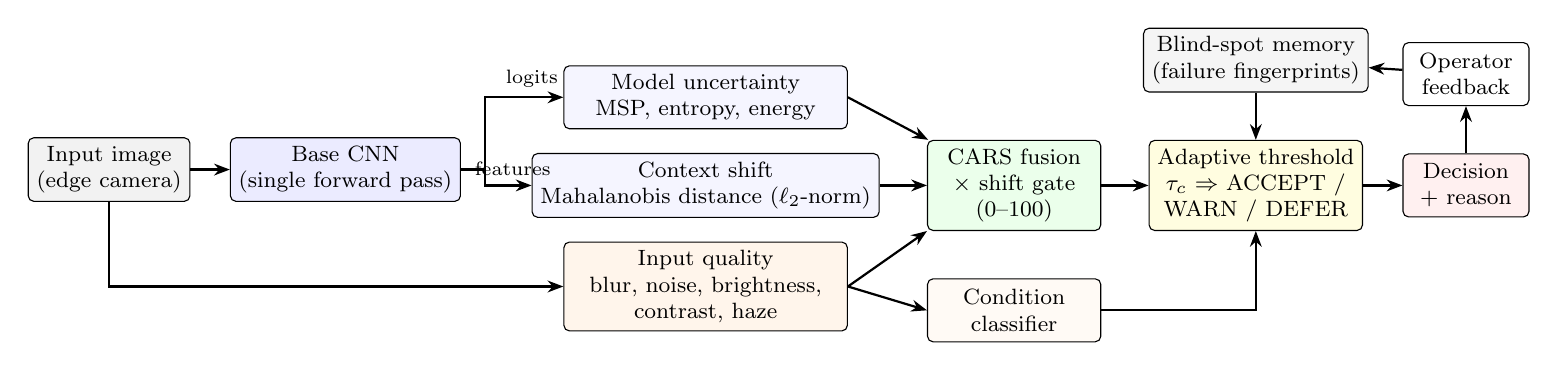
\begin{tikzpicture}[
  font=\footnotesize,
  box/.style={draw, rounded corners=2pt, align=center, minimum height=8mm, inner sep=3pt, fill=#1},
  box/.default=white,
  arr/.style={-{Stealth[length=2mm]}, thick},
  node distance=4mm and 5mm]
\node[box=gray!10, minimum width=17mm] (img) {Input image\\(edge camera)};
\node[box=blue!8, right=of img, minimum width=22mm] (cnn) {Base CNN\\(single forward pass)};
\node[box=blue!4, above right=1mm and 13mm of cnn, minimum width=36mm] (mu) {Model uncertainty\\ MSP, entropy, energy};
\node[box=blue!4, below=3mm of mu, minimum width=36mm] (cs) {Context shift\\ Mahalanobis distance ($\ell_2$-norm)};
\node[box=orange!8, below=3mm of cs, minimum width=36mm] (iq) {Input quality\\ blur, noise, brightness,\\ contrast, haze};
\node[box=green!8, right=6mm of cs, minimum width=22mm] (cars) {CARS fusion\\ $\times$ shift gate\\ (0--100)};
\node[box=orange!4, below=6mm of cars, minimum width=22mm] (cond) {Condition\\ classifier};
\node[box=yellow!12, right=6mm of cars, minimum width=25mm] (dec) {Adaptive threshold\\ $\tau_c$ $\Rightarrow$ ACCEPT /\\ WARN / DEFER};
\node[box=red!6, right=5mm of dec, minimum width=16mm] (out) {Decision\\ + reason};
\node[box=gray!8, above=6mm of dec, minimum width=26mm] (mem) {Blind-spot memory\\ (failure fingerprints)};
\node[box=white, above=6mm of out, minimum width=16mm] (op) {Operator\\ feedback};
\draw[arr] (img) -- (cnn);
\draw[arr] (cnn.east) -- ++(3mm,0) |- (mu.west) node[pos=0.8, above, font=\scriptsize]{logits};
\draw[arr] (cnn.east) -- ++(3mm,0) |- (cs.west) node[pos=0.8, above, font=\scriptsize]{features};
\draw[arr] (img.south) |- (iq.west);
\draw[arr] (mu.east) -- (cars);
\draw[arr] (cs.east) -- (cars);
\draw[arr] (iq.east) -- (cars.south west);
\draw[arr] (iq.east) -- (cond.west);
\draw[arr] (cars) -- (dec);
\draw[arr] (cond.east) -| (dec.south);
\draw[arr] (dec) -- (out);
\draw[arr] (mem) -- (dec);
\draw[arr] (out) -- (op);
\draw[arr] (op) -- (mem);
\end{tikzpicture}
\caption{EdgeGuard pipeline. One forward pass supplies the logits and features; image statistics come directly from the pixels. The fused score, the condition-specific threshold and the blind-spot memory produce the decision and its reason.}
\label{fig:pipeline}
\end{figure*}

\subsection{Single-Pass Reliability Signals}

EdgeGuard groups its evidence into the three factors of the problem statement: whether the model is unsure, whether the input looks unlike the training data, and whether the image is degraded. Each signal is one scalar per image.

\subsubsection{Model uncertainty}
For logits $\mathbf{z}\in\mathbb{R}^{C}$ and softmax probabilities $p_k$, EdgeGuard uses the maximum softmax probability (MSP), the entropy and the energy score \cite{hendrycks2017baseline,liu2020energy}:
\begin{equation}
s_{\text{msp}}=\max_k p_k,\quad s_{\text{ent}}=-\sum_{k} p_k\log p_k,\quad s_{\text{E}}=-\log\sum_{k} e^{z_k}.
\label{eq:logit}
\end{equation}

\subsubsection{Context shift}
With penultimate features $\mathbf{f}\in\mathbb{R}^{D}$ and $\tilde{\mathbf{f}}=\mathbf{f}/\lVert\mathbf{f}\rVert_2$, class means $\boldsymbol{\mu}_c$ and a shared covariance are fitted once on training features \cite{lee2018mahalanobis}, with shrinkage $\lambda=10^{-3}$:
\begin{equation}
\boldsymbol{\Sigma}=\mathbf{S}+\tfrac{\lambda\,\mathrm{tr}(\mathbf{S})}{D}\mathbf{I},\quad \mathbf{S}=\tfrac{1}{N}\textstyle\sum_{i}(\tilde{\mathbf{f}}_i-\boldsymbol{\mu}_{y_i})(\tilde{\mathbf{f}}_i-\boldsymbol{\mu}_{y_i})^{\top}.
\label{eq:cov}
\end{equation}
The signals are the distance to the closest class and the raw feature norm,
\begin{equation}
s_{\text{M}}=\log\min_{c}\sqrt{(\tilde{\mathbf{f}}-\boldsymbol{\mu}_c)^{\top}\boldsymbol{\Sigma}^{-1}(\tilde{\mathbf{f}}-\boldsymbol{\mu}_c)},\qquad s_{\text{N}}=\log\lVert\mathbf{f}\rVert_2 ,
\label{eq:maha}
\end{equation}
which cost one $D\times D$ and one $D\times C$ product at run time.

\subsubsection{Input quality}
On the grey image $I$ of size $H\times W$, sharpness is $s_{\text{B}}=\log(1+\mathrm{Var}(\nabla^{2}I))$ \cite{pechpacheco2000autofocus} and noise follows Immerkær \cite{immerkaer1996noise},
\begin{equation}
s_{\sigma}=\sqrt{\pi/2}\;\frac{1}{6(W-2)(H-2)}\sum_{x,y}\bigl|(I*\mathbf{N})(x,y)\bigr|,
\label{eq:noise}
\end{equation}
with $\mathbf{N}=[1,-2,1;-2,4,-2;1,-2,1]$. Brightness and contrast are the mean and standard deviation of $I/255$, and haze is the mean dark channel \cite{he2009darkchannel}. All five take about 26\,$\mu$s per $32\times32$ image on one core.

\subsection{Context-Aware Reliability Score}

The ten standardised signals $\mathbf{s}$ feed a logistic model of the probability that the base prediction is wrong, $p_{\text{fail}}=\sigma(\mathbf{w}^{\top}\mathbf{s}+b)$. It is trained only on in-distribution images, clean and degraded, and never sees OOD data. So that novelty is not under-weighted, a gate pushes the score towards zero once the feature distance leaves the range seen on clean calibration images:
\begin{equation}
g=\sigma\!\left(\frac{s_{\text{M}}-q_{99}}{\kappa}\right),\qquad \text{CARS}=100\,(1-p_{\text{fail}})(1-g),
\label{eq:cars}
\end{equation}
where $q_{99}$ is the 99th percentile of $s_{\text{M}}$ on clean calibration data and $\kappa$ is a quarter of its inter-quartile range.

\subsection{Adaptive Thresholds and Decision Policy}

The same score carries a different error rate in daylight and in fog, so EdgeGuard first detects the imaging condition and then applies a threshold tuned for it.

\subsubsection{Condition detection}
A multinomial logistic regression on the five quality statistics assigns each input to normal, noise, blur, low light or fog. It is trained on calibration images whose degradation is known.

\subsubsection{Threshold selection}
For condition $c$, calibration samples are sorted by CARS. If the top $n$ contain $k$ failures, their one-sided Clopper--Pearson bound \cite{clopper1934binomial} is $U(k,n)=\mathrm{Beta}^{-1}(0.9;\,k+1,\,n-k)$, and $\tau_c$ is the lowest CARS for which $U\le\varepsilon=3\%$ with $n\ge30$. Rarely seen conditions get a wider bound and thus a stricter threshold, without hand tuning.

\subsubsection{Decision rule}
For detected condition $\hat{c}$,
\begin{equation}
a=\begin{cases}
\text{ACCEPT}, & \text{CARS}\ge\tau_{\hat{c}},\\
\text{WARN}, & 50\le\text{CARS}<\tau_{\hat{c}},\\
\text{DEFER}, & \text{CARS}<50,
\end{cases}
\label{eq:decision}
\end{equation}
where WARN means act with caution or request another frame, and DEFER hands the input to a backup model or a person.

\subsection{Failure Reason and Blind-Spot Memory}

A flag is useful only if the operator knows what to fix, and repeated mistakes should become easier to catch. Two light components serve these needs.

\subsubsection{Failure reason}
For each WARN or DEFER, a degradation is reported if the condition classifier is at least 50\% confident in it. Otherwise ``unknown object'' is reported if $s_{\text{M}}$ exceeds the 95th clean percentile or the gate is active, and the remaining cases are labelled ambiguous.

\subsubsection{Blind-spot memory}
When an operator confirms a wrong prediction, $\tilde{\mathbf{f}}$ is stored in float16 with the predicted class in a first-in, first-out bank of 512 entries (132\,KB); no image is kept. If a new input's cosine similarity to a stored failure of the same predicted class exceeds $\tau_{\mathcal{M}}=0.955$, chosen so that 5\% of correct calibration predictions would trigger it, an ACCEPT becomes WARN. Algorithm~\ref{alg:infer} summarises the inference path.

\begin{algorithm}[t]
\caption{EdgeGuard single-pass inference}
\label{alg:infer}
\begin{algorithmic}[1]
\Require Image $x$, calibrated EdgeGuard, memory $\mathcal{M}$
\Ensure Prediction $\hat{y}$, CARS, action $a$, reason $r$
\State $(\mathbf{z},\mathbf{f})\gets h(x)$; $\hat{y}\gets\arg\max\mathbf{z}$ \Comment{only network pass}
\State Compute $\mathbf{s}$ from $\mathbf{z}$, $\mathbf{f}$ and the pixels of $x$
\State $\text{CARS}\gets100(1-p_{\text{fail}})(1-g)$ \Comment{Eq.~(\ref{eq:cars})}
\State $\hat{c}\gets$ condition classifier$(\mathbf{s})$; $a\gets$ Eq.~(\ref{eq:decision}) with $\tau_{\hat{c}}$
\If{$a=\text{ACCEPT}$ \textbf{and} $\max_{m\in\mathcal{M},\,y_m=\hat{y}}\cos(\tilde{\mathbf{f}},m)\ge\tau_{\mathcal{M}}$}
  \State $a\gets\text{WARN}$; $r\gets$ ``matches a past failure''
\ElsIf{$a\neq\text{ACCEPT}$}
  \State $r\gets$ condition $\rightarrow$ unknown object $\rightarrow$ ambiguous
\EndIf
\If{operator confirms $\hat{y}$ is wrong}
  \State add $(\tilde{\mathbf{f}},\hat{y})$ to $\mathcal{M}$
\EndIf
\State \Return $\hat{y}$, CARS, $a$, $r$
\end{algorithmic}
\end{algorithm}

\subsection{Implementation Details}

EdgeGuard was implemented in Python with PyTorch, OpenCV and scikit-learn. The components below describe the experimental setup and match the released code.

\subsubsection{Network and training}
EdgeNet, the reference classifier, has six $3\times3$ convolution layers (widths 32, 32, 64, 64, 128, 128) with batch normalisation, ReLU and max pooling after every second layer, then global average pooling to 128 features, dropout ($p=0.3$) and a linear layer, for 288{,}746 parameters. CIFAR-10 \cite{krizhevsky2009cifar} was split into 45{,}000 training and 5{,}000 calibration images. Training used SGD with Nesterov momentum 0.9, weight decay $5\times10^{-4}$, batch size 128 and a one-cycle schedule peaking at 0.05 for 20 epochs, with random crops and flips, and reached 84.8\% clean test accuracy.

\subsubsection{Calibration and test data}
Each calibration image was used clean and under Gaussian noise, defocus blur, low light and fog at a random severity from 1 to 5, giving 25{,}000 samples with a 38.1\% failure rate. Eight corruptions were re-implemented in the style of CIFAR-10-C \cite{hendrycks2019corruptions} at five severities; shot noise, motion blur, contrast and JPEG were never used for calibration. Two OOD sets of 2{,}000 images were generated: rendered house-number digits in the style of SVHN \cite{netzer2011svhn} and texture crops in the style of DTD \cite{cimpoi2014dtd}. The test set thus held 10{,}000 clean, 80{,}000 corrupted and 4{,}000 OOD images.

\subsubsection{Baselines and metrics}
EdgeGuard was compared with MSP \cite{hendrycks2017baseline}, entropy, energy \cite{liu2020energy}, the normalised Mahalanobis distance alone \cite{lee2018mahalanobis} and MC dropout \cite{gal2016dropout} with 20 samples, all on the same network. Metrics were AUROC, AUPR with failures as positives, FPR at 95\% recall (FPR95), 15-bin expected calibration error (ECE) \cite{guo2017calibration}, the area under the risk--coverage curve (AURC) \cite{geifman2017selective}, coverage, error on accepted inputs and false-alarm rates.

\subsubsection{Deployment and hardware}
The scaler and both logistic models were folded into plain weight vectors, and the network was exported to ONNX (1.16\,MB). Experiments ran on two CPU cores with 8\,GB of RAM and no GPU; latency is the median of 192 single-image runs on one thread.

\subsection{Challenges Encountered and Solutions}

Several design choices came from problems found during development rather than from the original plan.

\subsubsection{Feature collapse}
On raw features, dark and low-contrast images collapsed towards the origin, close to every class mean, and the Mahalanobis OOD AUROC was only 0.49 to 0.67. Normalising features before fitting raised it to 0.94 to 0.97, and the norm was kept as a separate signal.

\subsubsection{Fusion that ignores novelty}
Trained on in-distribution failures only, the fusion under-weighted the shift signal and detected OOD inputs worse than Mahalanobis alone (0.926 against 0.971 on digits). The gate in Eq.~(\ref{eq:cars}) lifted it to 0.960 without any OOD data.

\subsubsection{Unstable thresholds and overhead}
Empirical error rates gave unstable thresholds for rare conditions, which the Clopper--Pearson bound fixed. Calling scikit-learn per image added about 2\,ms, more than the network itself; folding the models into NumPy weights cut the post-forward step to 0.14\,ms.

% ---------------------------------------------------------------------------
\section{Results and Analysis}
\label{sec:results}

This section first shows why reliability estimation is needed, then compares detection, calibration and decisions with the baselines, and closes with ablation, efficiency and limitations.

\subsection{Accuracy Under Distribution Shift}

As Fig.~\ref{fig:severity} shows, mean accuracy fell from 84.8\% on clean images to 77.6\% at severity 1 and 35.1\% at severity 5, with contrast (34.8\%), motion blur (41.4\%) and low light (43.9\%) the most damaging. The drop was as steep on corruptions never used for calibration. Over all 94{,}000 inputs the unguarded model was wrong 43.5\% of the time, and 5.7\% of its errors carried a softmax confidence of 0.9 or more.

\begin{figure}[t]
\centering
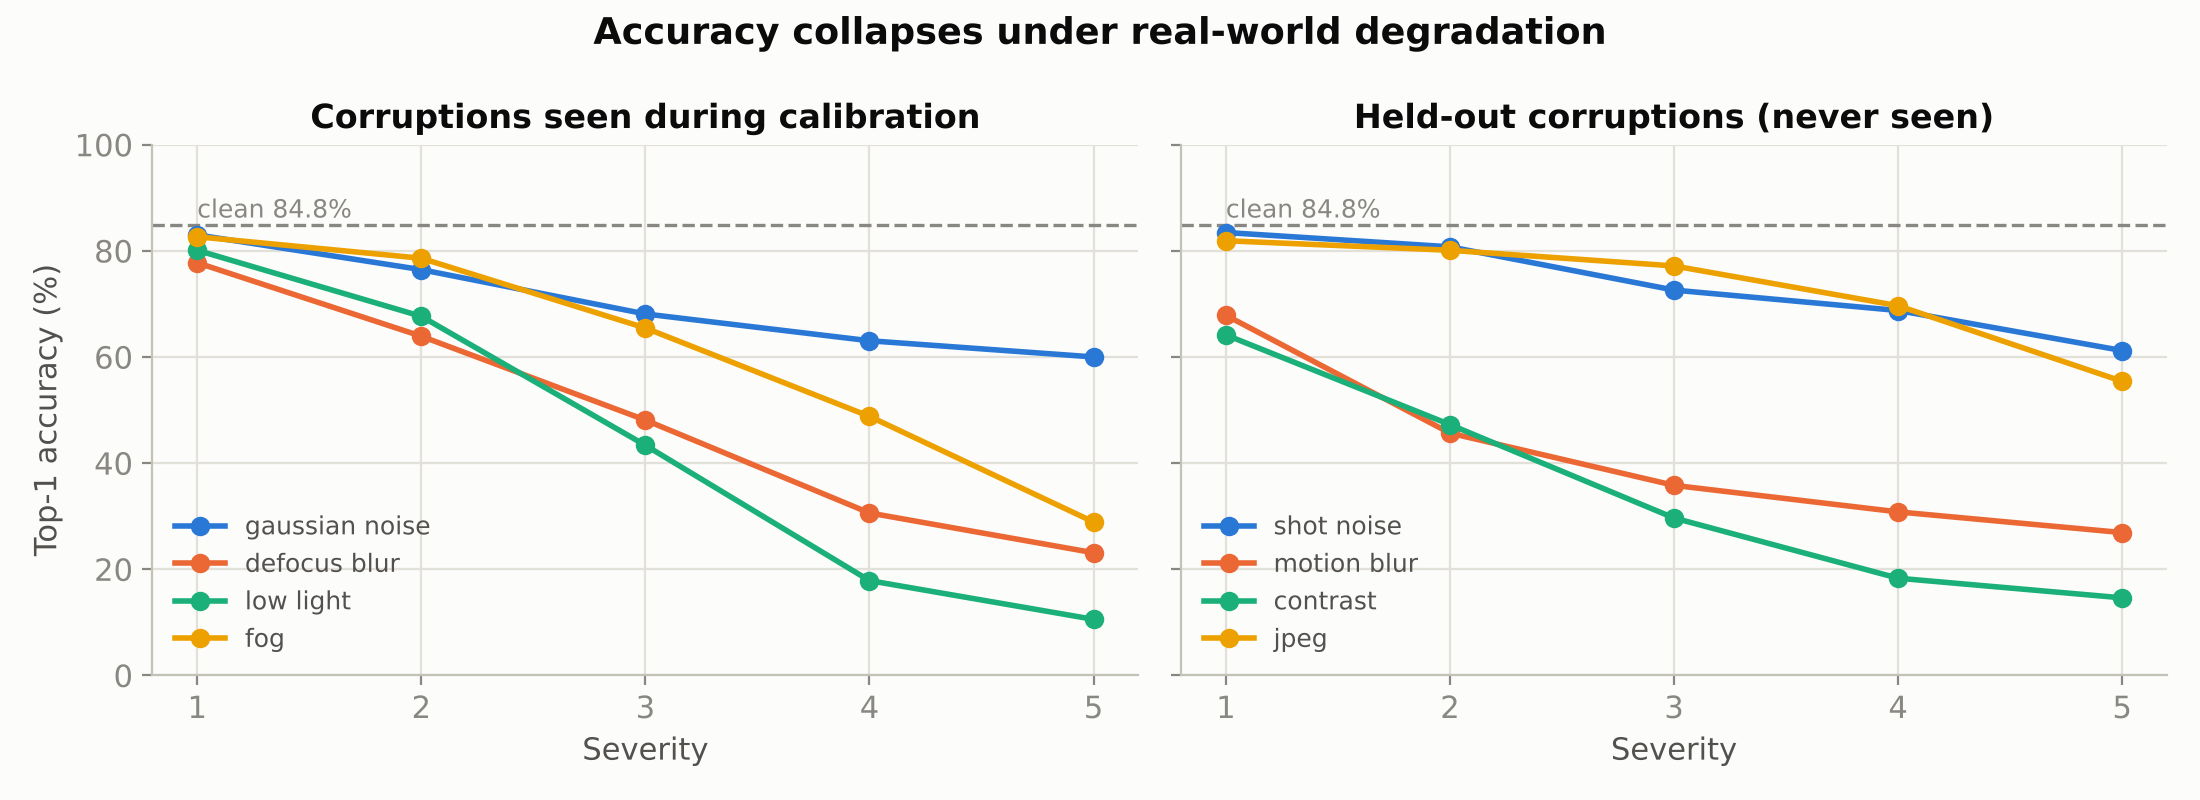
\includegraphics[width=\columnwidth]{fig02_accuracy_vs_severity.png}
\caption{Accuracy of the base model against corruption severity, for corruptions used in calibration (left) and unseen corruptions (right).}
\label{fig:severity}
\end{figure}

\subsection{Failure and Out-of-Distribution Detection}

Table~\ref{tab:detection} compares how well each score ranked unreliable inputs. For wrong predictions on clean and corrupted images, CARS reached the best AUROC (0.842) and AUPR (0.756), slightly above MSP (0.837) and MC dropout (0.836), and the ordering held on unseen corruptions. The gain in ranking failures was small. For novel inputs it was larger: OOD AUROC rose from 0.866 to 0.960 on digits and from 0.842 to 0.910 on textures relative to MSP. Mahalanobis alone was the best OOD detector but the weakest failure detector (0.800), so neither signal suffices on its own.

\begin{table*}[t]
\centering
\caption{Failure detection (wrong predictions on clean and corrupted inputs) and OOD detection. Digits and Textures give OOD AUROC; the last column gives FPR95 on digits.}
\label{tab:detection}
\footnotesize
\setlength{\tabcolsep}{4pt}
\begin{tabular}{lcccccccc}
\toprule
 & & \multicolumn{3}{c}{Failure, all corruptions} & Unseen & \multicolumn{3}{c}{OOD detection} \\
\cmidrule(lr){3-5}\cmidrule(lr){6-6}\cmidrule(lr){7-9}
Method & Passes & AUROC$\uparrow$ & AUPR$\uparrow$ & FPR95$\downarrow$ & AUROC$\uparrow$ & Digits$\uparrow$ & Textures$\uparrow$ & FPR95$\downarrow$ \\
\midrule
MSP \cite{hendrycks2017baseline} & 1 & 0.837 & 0.737 & 0.480 & 0.843 & 0.866 & 0.842 & 0.385 \\
Entropy & 1 & 0.838 & 0.741 & \textbf{0.477} & 0.846 & 0.882 & 0.860 & 0.376 \\
Energy \cite{liu2020energy} & 1 & 0.818 & 0.724 & 0.554 & 0.827 & 0.884 & 0.874 & 0.336 \\
Mahalanobis (normalised) \cite{lee2018mahalanobis} & 1 & 0.800 & 0.723 & 0.633 & 0.804 & \textbf{0.971} & \textbf{0.937} & \textbf{0.148} \\
MC dropout \cite{gal2016dropout} & 20 (head) & 0.836 & 0.738 & 0.482 & 0.844 & 0.881 & 0.858 & 0.366 \\
\textbf{EdgeGuard CARS} & 1 & \textbf{0.842} & \textbf{0.756} & 0.483 & \textbf{0.848} & 0.960 & 0.910 & 0.206 \\
\bottomrule
\end{tabular}
\end{table*}

\subsection{Calibration and Decisions}

Fig.~\ref{fig:calib} shows that softmax confidence was over-confident on corrupted inputs (ECE 12.5\%), whereas EdgeGuard's estimate $1-p_{\text{fail}}$ stayed near the diagonal (ECE 4.2\%); on clean images the two were similar (1.9\% and 2.2\%). Selective-prediction ranking changed little (AURC 0.169 against 0.170 for MSP).

\begin{figure}[t]
\centering
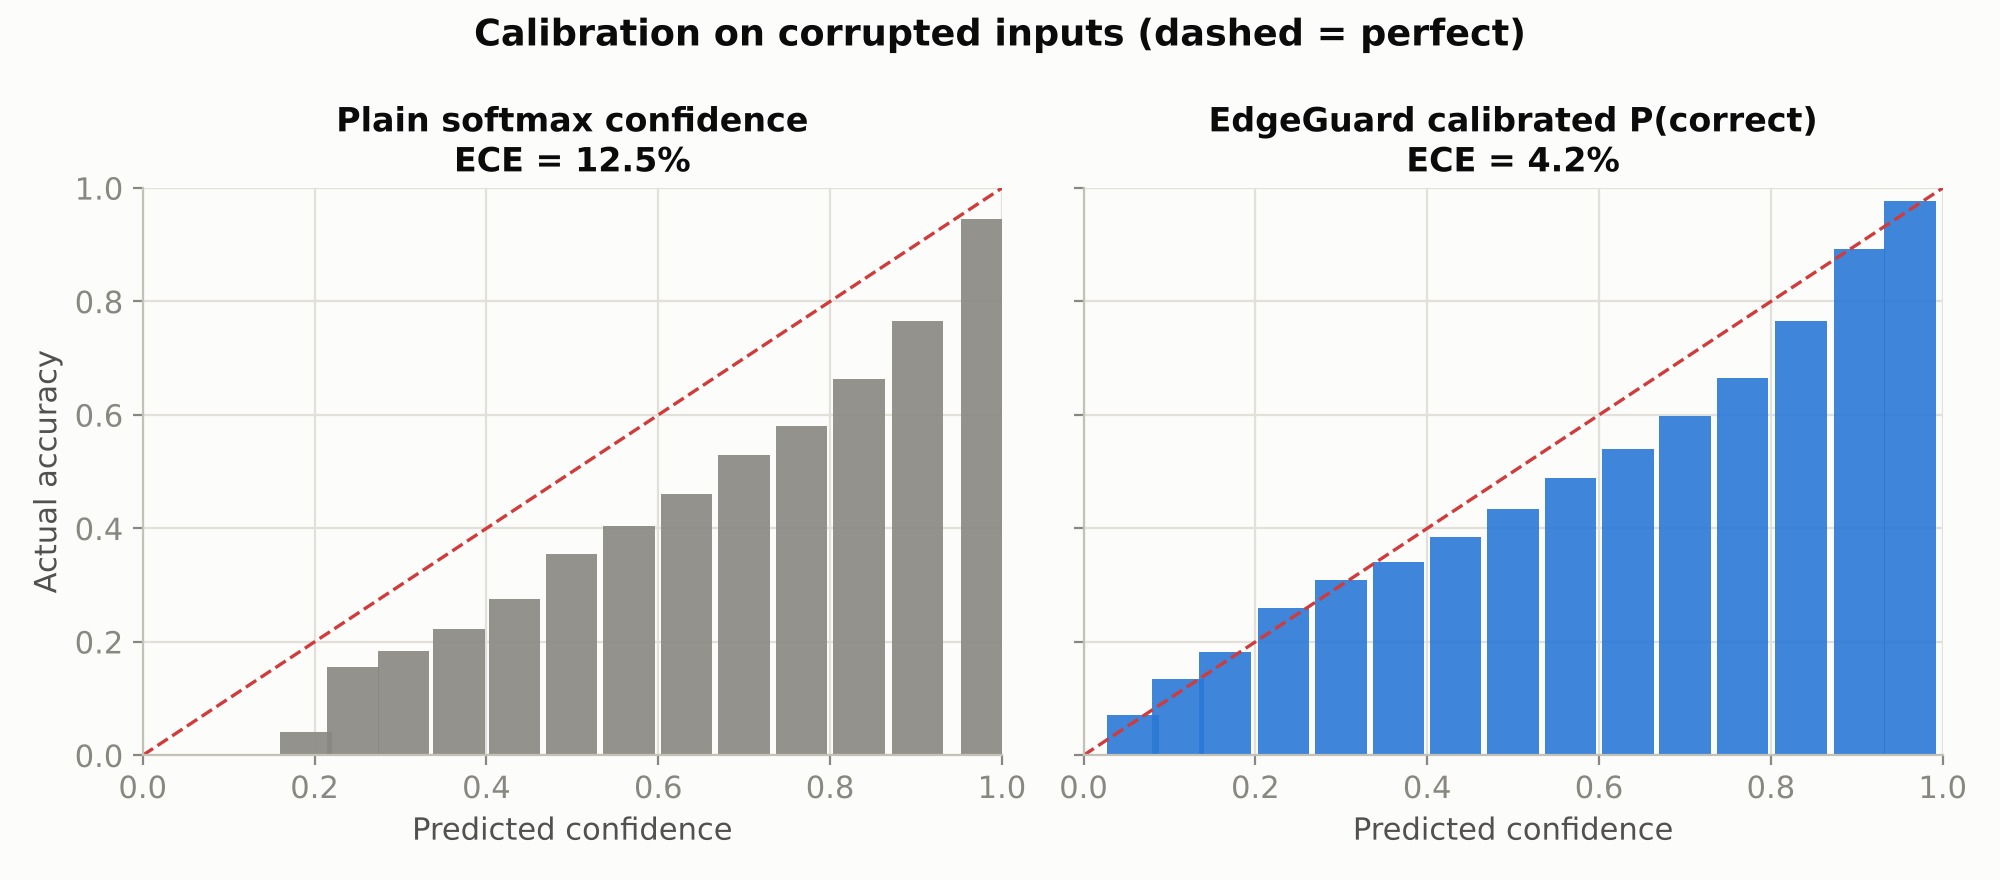
\includegraphics[width=\columnwidth]{fig06_reliability_diagram.png}
\caption{Reliability diagrams on corrupted inputs: softmax confidence (left) and EdgeGuard's calibrated probability of a correct prediction (right).}
\label{fig:calib}
\end{figure}

Table~\ref{tab:decisions} summarises the three-way decisions. Over all inputs EdgeGuard accepted 22.7\% of predictions with 3.5\% error, against 43.5\% when every prediction was acted on, and flagged 98.2\% of failures. On clean images it accepted 59.4\% with 2.8\% error, against 15.2\%. The cost was a high soft-alarm rate: 31.9\% of correct clean predictions received WARN or DEFER, although only 5.4\% were deferred. Fig.~\ref{fig:decisions} shows that decisions followed input difficulty, with almost nothing accepted under severe blur, low light or fog and 87\% of unknown digits deferred.

\begin{table}[t]
\centering
\caption{Decision-level results with adaptive thresholds ($\varepsilon=3\%$).}
\label{tab:decisions}
\small
\setlength{\tabcolsep}{4pt}
\begin{tabular}{lcc}
\toprule
Metric & Clean only & All 94k inputs \\
\midrule
Error of unguarded model & 15.2\% & 43.5\% \\
Coverage (ACCEPT) & 59.4\% & 22.7\% \\
Error on accepted inputs & \textbf{2.8\%} & \textbf{3.5\%} \\
Failures flagged (recall) & 89.0\% & 98.2\% \\
Correct inputs deferred & 5.4\% & 21.5\% \\
Correct inputs warned/deferred & 31.9\% & 61.3\% \\
\bottomrule
\end{tabular}
\end{table}

\begin{figure}[t]
\centering
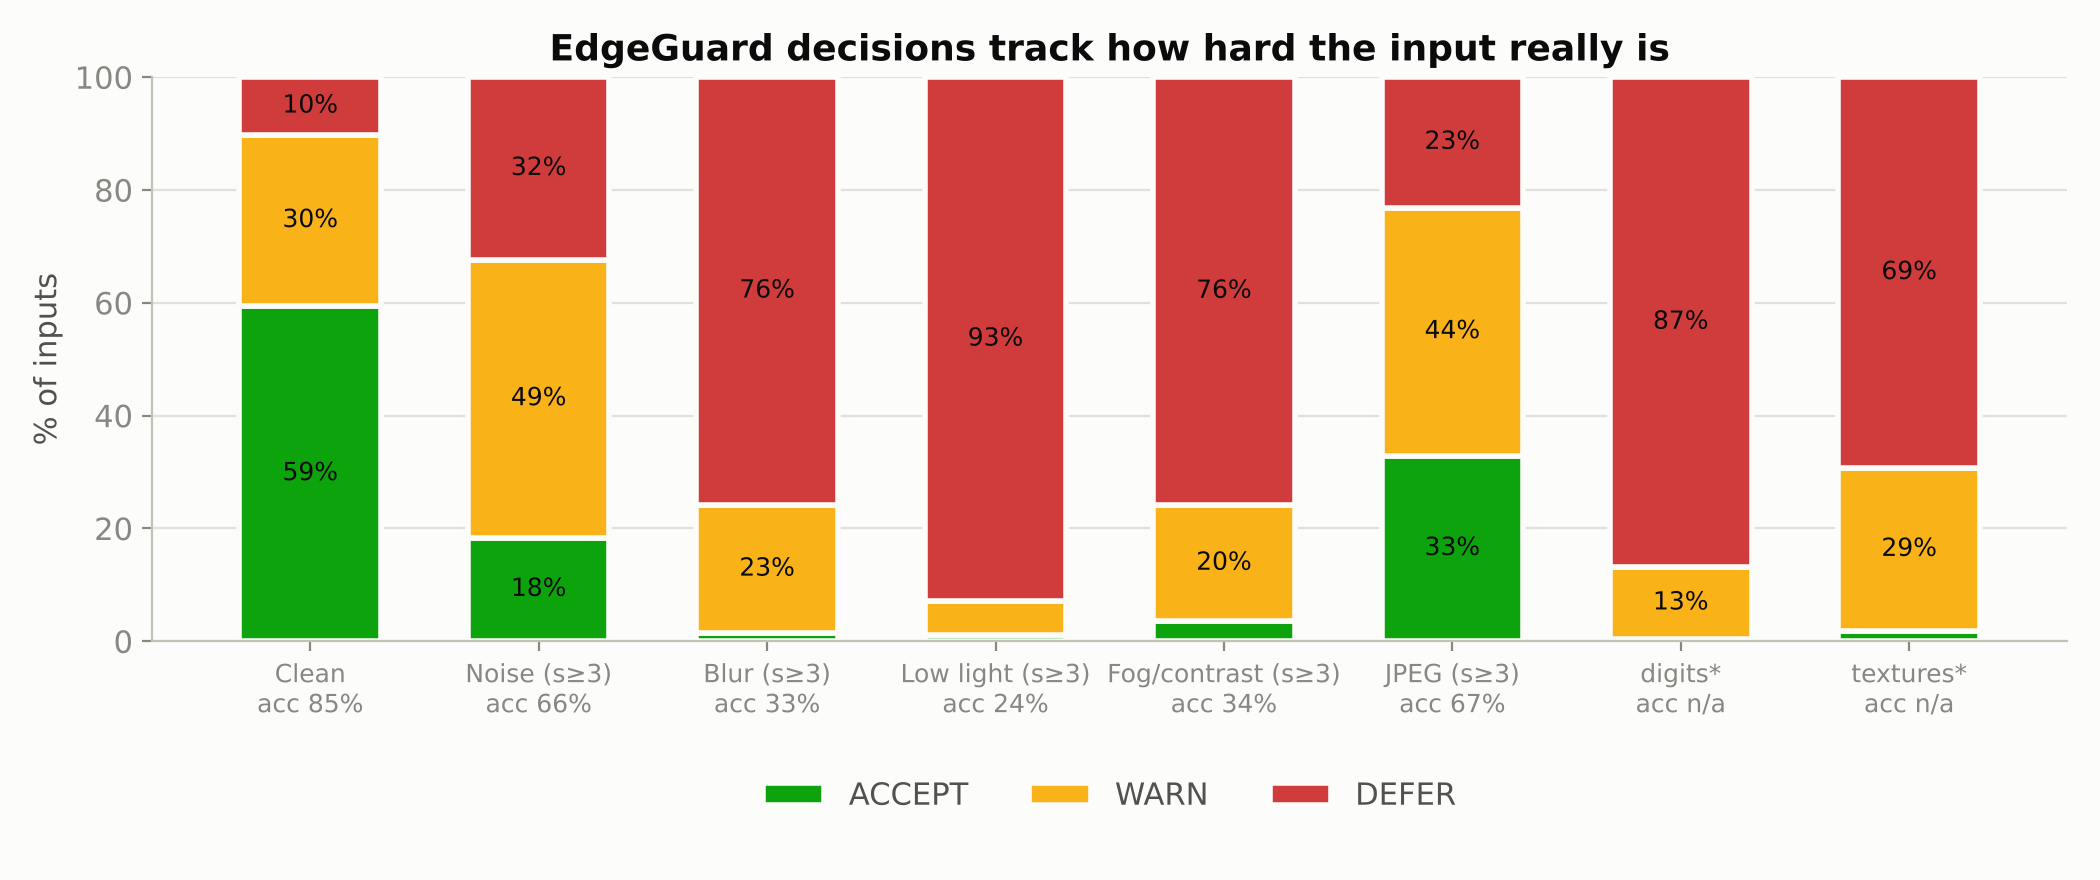
\includegraphics[width=\columnwidth]{fig08_decision_breakdown.png}
\caption{Share of ACCEPT, WARN and DEFER decisions by input condition (severity 3 to 5). Digits and textures are the OOD sets.}
\label{fig:decisions}
\end{figure}

\subsection{Adaptive Thresholds, Explanations and Memory}

The calibrated thresholds were 88.6 for normal images, about 92 for noise, blur and fog, and 86.1 for low light, against a single fixed threshold of 89.6. Compared with the fixed threshold, they lowered the error on accepted noisy images from 5.2\% to 3.1\% and on foggy images from 4.9\% to 3.7\%, but accepted blurred images were still wrong 19.8\% of the time, mostly under unseen motion blur, and accepted JPEG images 6.8\%. Overall the error on accepted predictions fell from 4.0\% to 3.5\% while coverage fell from 24.4\% to 22.7\%.

For flagged inputs with a known cause, the primary reason matched the truth in 86.1\% of 43{,}084 cases: 99.5\% for noise, 93.7\% for blur, 100\% for low light and 77.2\% for fog. Unknown objects were named first in only 35.0\% of cases because many were also dark or low in contrast, though the OOD flag was raised as a secondary reason for 55.0\%. Fig.~\ref{fig:examples} shows typical outputs.

The blind-spot memory was tested on two streams of 3{,}000 images, half clean and half under an unseen shift, with every flagged failure and 30\% of silent misses confirmed by a simulated operator. Silent misses fell from 2.36\% to 1.95\% of failures under motion blur and from 7.04\% to 6.20\% under JPEG, reductions of 17\% and 12\%, while false alarms rose by 3.1 and 2.1 points. The benefit is real but modest and depends on how much feedback operators give.

\begin{figure*}[t]
\centering
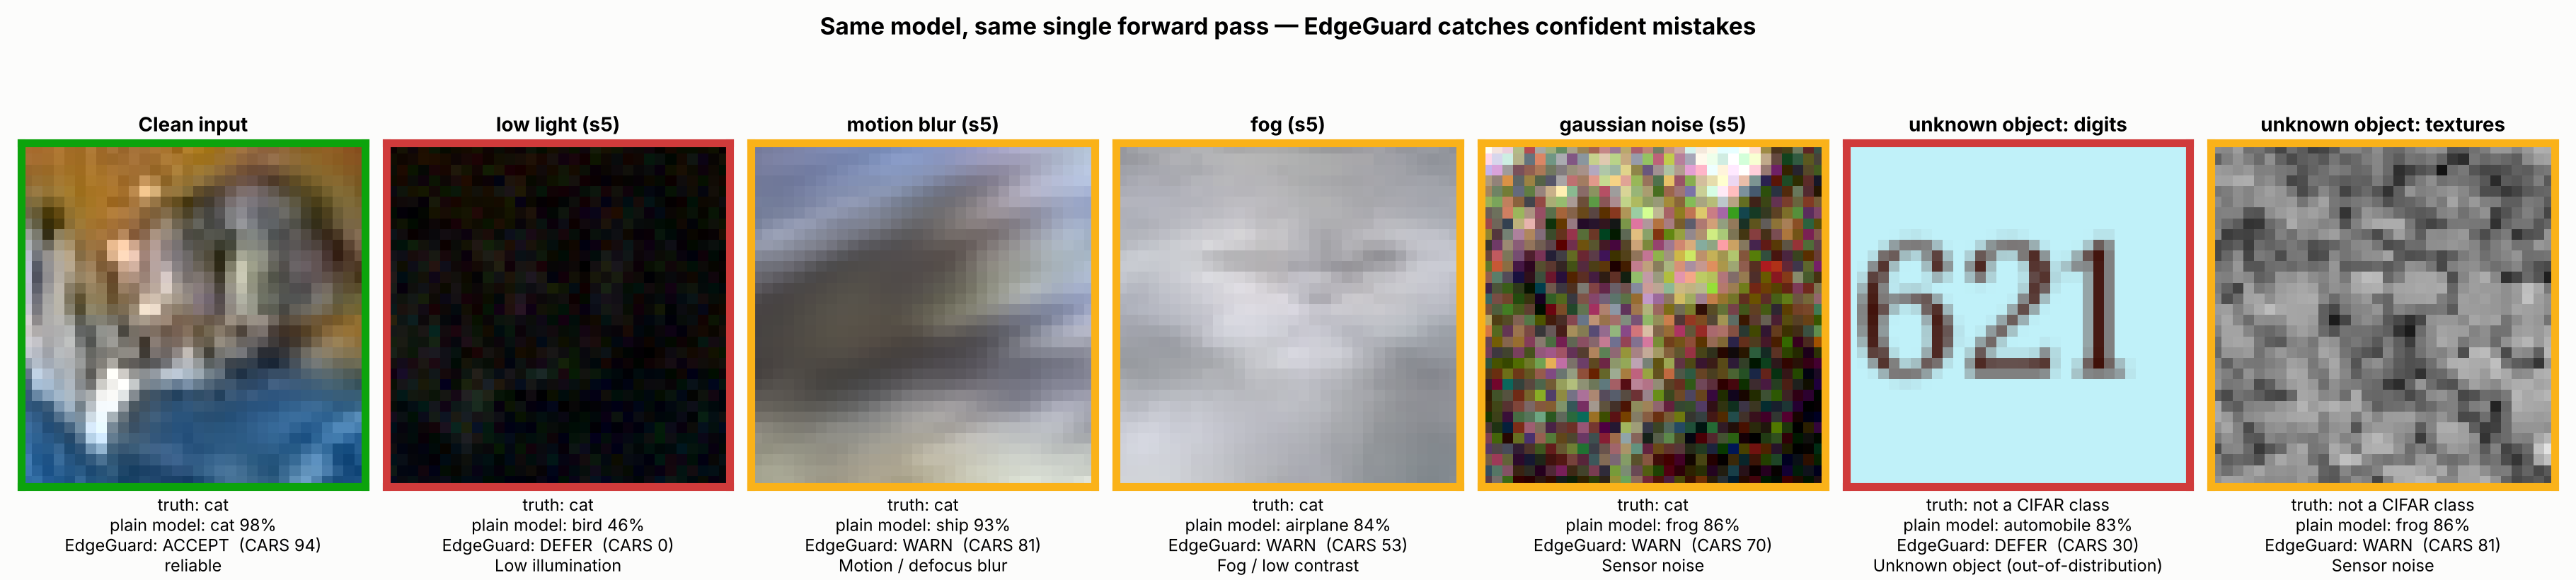
\includegraphics[width=\textwidth]{fig00_examples.png}
\caption{Example outputs. The plain model is confidently wrong under several degradations and on unknown objects; EdgeGuard flags the same predictions and names a cause (frame colour: green ACCEPT, amber WARN, red DEFER).}
\label{fig:examples}
\end{figure*}

\subsection{Ablation and Edge Efficiency}

Table~\ref{tab:ablation} refits the fusion on subsets of signals. Model uncertainty alone gave 0.835 AUROC on unreliable inputs; adding context shift mainly helped OOD detection (0.872 to 0.935), and input quality added a small gain on unseen corruptions. Input quality alone was clearly insufficient.

\begin{table}[t]
\centering
\caption{Ablation of signal groups (AUROC). ``Unreliable'' counts wrong predictions and OOD inputs.}
\label{tab:ablation}
\small
\setlength{\tabcolsep}{4pt}
\begin{tabular}{lccc}
\toprule
Signals used & Unreliable & Unseen corr. & OOD \\
\midrule
Model uncertainty & 0.835 & 0.846 & 0.872 \\
+ Context shift & 0.844 & 0.846 & \textbf{0.935} \\
+ Input quality (full) & \textbf{0.845} & \textbf{0.848} & \textbf{0.935} \\
Input quality only & 0.704 & 0.726 & 0.730 \\
\bottomrule
\end{tabular}
\end{table}

As Table~\ref{tab:efficiency} shows, EdgeGuard added 0.14\,ms to a 2.31\,ms PyTorch forward pass (5.9\%) and 14.3\% relative to the 0.95\,ms ONNX Runtime pass, within the 10 to 15\% budget set for the project, while ten-pass MC dropout took 19.0\,ms. The extra memory was 70\,KB, plus 132\,KB for a full failure memory.

\begin{table}[t]
\centering
\caption{Latency per image (one CPU thread, batch 1) and extra memory.}
\label{tab:efficiency}
\small
\setlength{\tabcolsep}{4pt}
\begin{tabular}{lcc}
\toprule
Method & Latency (ms) & Extra memory \\
\midrule
Base network (PyTorch / ONNX) & 2.31 / 0.95 & -- \\
\textbf{EdgeGuard (PyTorch base)} & \textbf{2.45} & 70\,KB + 132\,KB \\
MC dropout, 10 passes & 19.0 & -- \\
Deep ensemble, 5 members & $\approx$11.6 & $5\times$ weights \\
\bottomrule
\end{tabular}
\end{table}

\subsection{Comparison with Existing Approaches}

Table~\ref{tab:compare} compares design properties, since prior methods report results on different benchmarks. EdgeGuard is the only one that combines single-pass operation, separate input-quality evidence, a stated reason for each flag and learning from deployment feedback without updating the network.

\begin{table}[t]
\centering
\caption{Design comparison with existing reliability approaches.}
\label{tab:compare}
\small
\setlength{\tabcolsep}{3pt}
\begin{tabular}{lcccc}
\toprule
Approach & Passes & Quality & Reason & Learns \\
\midrule
MC dropout \cite{gal2016dropout} & $T$ & -- & -- & -- \\
Deep ensembles \cite{lakshminarayanan2017ensembles} & $M$ nets & -- & -- & -- \\
TULiP \cite{zhang2025tulip} & $\approx$10 & -- & -- & -- \\
Mahalanobis \cite{lee2018mahalanobis} & 1 & -- & -- & -- \\
Energy-aware NECO \cite{zhang2026neco} & 1 & -- & -- & -- \\
On-device TTA \cite{danilowski2026botta} & 1+grad & -- & -- & weights \\
\textbf{EdgeGuard} & \textbf{1} & \textbf{yes} & \textbf{yes} & \textbf{memory} \\
\bottomrule
\end{tabular}
\end{table}

\subsection{Relation to Objectives and Limitations}

The objectives set for the project were met: the model estimates its own reliability, the module works in a single pass with 0.14\,ms overhead and 70\,KB of extra parameters, the evaluation covered clean, corrupted, unseen and OOD inputs, and accuracy was untouched while 98.2\% of failures were flagged. Several limitations remain. The reference network is small (84.8\% clean accuracy), which inflates error rates and warnings. The corruptions were re-implemented and the OOD sets were generated proxies rather than CIFAR-10-C, CIFAR-100 or SVHN, which could not be downloaded in our environment. CARS improved only slightly over softmax at ranking misclassifications, the adaptive thresholds missed the 3\% target on blur and unseen JPEG, the memory relies on operator feedback, and latency was measured on a general-purpose CPU rather than an embedded board.

% ---------------------------------------------------------------------------
\section{Conclusion and Future Work}
\label{sec:conclusion}

This paper presented EdgeGuard, a reliability layer that gives an unmodified image classifier a calibrated sense of when not to trust its predictions, using only the forward pass it already performs. By keeping model uncertainty, context shift and input quality separate before fusing them, EdgeGuard flagged 98.2\% of incorrect predictions on a demanding mix of corrupted and unfamiliar inputs, reduced the error of accepted predictions from 43.5\% to 3.5\%, raised OOD AUROC from 0.866 to 0.960 and lowered calibration error on corrupted inputs from 12.5\% to 4.2\%, for 0.14\,ms per image. Each flag came with a reason that matched the true cause in 86\% of cases. The gains in ranking ordinary misclassifications were small, and unseen motion blur still slipped past the thresholds more often than intended. For practitioners, the results suggest treating edge reliability as a decision problem: image quality and feature novelty are cheap enough to measure on every frame, and per-condition thresholds should come from an explicit statistical bound rather than hand tuning.

Future work will repeat the evaluation with a ResNet-18 backbone on the released CIFAR-10-C corruptions and on CIFAR-100 and SVHN, and will measure latency and energy on a Raspberry Pi and an NVIDIA Jetson board. The condition classifier can be extended to rain, glare and lens occlusion so that fewer shifts reach the thresholds unrecognised, and the same signals can be carried over to object detection and segmentation. Pairing the blind-spot memory with selective labelling would also let the failures it stores drive later retraining, closing the loop between deployment and model improvement.

% ---------------------------------------------------------------------------
\section*{Acknowledgment}
The authors thank the School of Computer Science and Engineering, KLE Technological University, Hubballi, for the facilities and guidance that supported this work.

% ---------------------------------------------------------------------------
\begin{thebibliography}{00}
\footnotesize

\bibitem{hendrycks2017baseline} D. Hendrycks and K. Gimpel, ``A baseline for detecting misclassified and out-of-distribution examples in neural networks,'' in \textit{Proc. ICLR}, 2017.

\bibitem{ovadia2019trust} Y. Ovadia \textit{et al.}, ``Can you trust your model's uncertainty? Evaluating predictive uncertainty under dataset shift,'' in \textit{Proc. NeurIPS}, 2019.

\bibitem{gal2016dropout} Y. Gal and Z. Ghahramani, ``Dropout as a Bayesian approximation: Representing model uncertainty in deep learning,'' in \textit{Proc. ICML}, 2016, pp. 1050--1059.

\bibitem{lakshminarayanan2017ensembles} B. Lakshminarayanan, A. Pritzel, and C. Blundell, ``Simple and scalable predictive uncertainty estimation using deep ensembles,'' in \textit{Proc. NeurIPS}, 2017.

\bibitem{zhang2025tulip} Y. Zhang, D. Wu, Y. Wada, and T. Kanamori, ``TULiP: Test-time uncertainty estimation via linearization and weight perturbation,'' in \textit{Proc. ICONIP}, 2025, pp. 476--491.

\bibitem{danilowski2026botta} M. Danilowski, S. Chatterjee, and A. Ghosh, ``BoTTA: Benchmarking on-device test time adaptation,'' in \textit{Proc. ACM SenSys}, 2026, pp. 465--477.

\bibitem{shao2023failure} W. Shao \textit{et al.}, ``Failure detection for motion prediction of autonomous driving: An uncertainty perspective,'' 2023.

\bibitem{rahmani2026edgecase} S. Rahmani \textit{et al.}, ``Edge case detection in automated driving: Methods, challenges and future directions,'' \textit{IEEE Trans. Intell. Transp. Syst.}, 2026.

\bibitem{guo2017calibration} C. Guo, G. Pleiss, Y. Sun, and K. Q. Weinberger, ``On calibration of modern neural networks,'' in \textit{Proc. ICML}, 2017, pp. 1321--1330.

\bibitem{liu2020energy} W. Liu, X. Wang, J. Owens, and Y. Li, ``Energy-based out-of-distribution detection,'' in \textit{Proc. NeurIPS}, 2020.

\bibitem{lee2018mahalanobis} K. Lee, K. Lee, H. Lee, and J. Shin, ``A simple unified framework for detecting out-of-distribution samples and adversarial attacks,'' in \textit{Proc. NeurIPS}, 2018.

\bibitem{vanamersfoort2020duq} J. van Amersfoort, L. Smith, Y. W. Teh, and Y. Gal, ``Uncertainty estimation using a single deep deterministic neural network,'' in \textit{Proc. ICML}, 2020.

\bibitem{liu2020sngp} J. Z. Liu \textit{et al.}, ``Simple and principled uncertainty estimation with deterministic deep learning via distance awareness,'' in \textit{Proc. NeurIPS}, 2020.

\bibitem{sensoy2018evidential} M. Sensoy, L. Kaplan, and M. Kandemir, ``Evidential deep learning to quantify classification uncertainty,'' in \textit{Proc. NeurIPS}, 2018.

\bibitem{yoon2024daedl} T. Yoon and H. Kim, ``Uncertainty estimation by density aware evidential deep learning,'' in \textit{Proc. ICML}, 2024.

\bibitem{azizmalayeri2024cea} M. Azizmalayeri, A. Abu-Hanna, and G. Cin\`{a}, ``Mitigating overconfidence in out-of-distribution detection by capturing extreme activations,'' in \textit{Proc. UAI}, 2024, pp. 203--224.

\bibitem{zhang2026neco} B. Zhang, H. Huang, and Y. Cao, ``Energy-aware NECO for single-pass pixel-wise out-of-distribution detection in semantic segmentation,'' in \textit{ICRA Workshop (LoWi)}, 2026.

\bibitem{mishra2025odd} A. Mishra and A. Liu, ``ODD: Overlap-aware estimation of model performance under distribution shift,'' in \textit{Proc. UAI}, 2025, pp. 3031--3047.

\bibitem{timans2025monitoring} A. Timans, R. Verma, E. Nalisnick, and C. A. Naesseth, ``On continuous monitoring of risk violations under unknown shift,'' in \textit{Proc. UAI}, 2025, pp. 4204--4226.

\bibitem{koebler2025incremental} A. Koebler, T. Decker, I. Thon, V. Tresp, and F. Buettner, ``Incremental uncertainty-aware performance monitoring with active labeling intervention,'' in \textit{Proc. AISTATS}, 2025, pp. 2188--2196.

\bibitem{ma2026embodi} X. Ma, Y. D. Kwon, and D. Ma, ``EmbodiTTA: Resource-efficient test-time adaptation for embodied visual systems,'' \textit{arXiv:2505.00986}, 2026.

\bibitem{hu2025duo} Z. Hu \textit{et al.}, ``Adaptive dual uncertainty optimization: Boosting monocular 3D object detection under test-time shifts,'' in \textit{Proc. ICCV}, 2025, pp. 7273--7283.

\bibitem{hendrycks2019corruptions} D. Hendrycks and T. Dietterich, ``Benchmarking neural network robustness to common corruptions and perturbations,'' in \textit{Proc. ICLR}, 2019.

\bibitem{lu2024oodsurvey} S. Lu \textit{et al.}, ``Out-of-distribution detection: A task-oriented survey of recent advances,'' 2024.

\bibitem{pechpacheco2000autofocus} J. L. Pech-Pacheco, G. Crist\'{o}bal, J. Chamorro-Mart\'{i}nez, and J. Fern\'{a}ndez-Valdivia, ``Diatom autofocusing in brightfield microscopy: A comparative study,'' in \textit{Proc. ICPR}, 2000, pp. 314--317.

\bibitem{immerkaer1996noise} J. Immerk\ae r, ``Fast noise variance estimation,'' \textit{Comput. Vis. Image Underst.}, vol. 64, no. 2, pp. 300--302, 1996.

\bibitem{he2009darkchannel} K. He, J. Sun, and X. Tang, ``Single image haze removal using dark channel prior,'' in \textit{Proc. CVPR}, 2009, pp. 1956--1963.

\bibitem{clopper1934binomial} C. J. Clopper and E. S. Pearson, ``The use of confidence or fiducial limits illustrated in the case of the binomial,'' \textit{Biometrika}, vol. 26, no. 4, pp. 404--413, 1934.

\bibitem{krizhevsky2009cifar} A. Krizhevsky, ``Learning multiple layers of features from tiny images,'' Univ. Toronto, Tech. Rep., 2009.

\bibitem{netzer2011svhn} Y. Netzer \textit{et al.}, ``Reading digits in natural images with unsupervised feature learning,'' in \textit{NIPS Workshop Deep Learn. Unsupervised Feature Learn.}, 2011.

\bibitem{cimpoi2014dtd} M. Cimpoi, S. Maji, I. Kokkinos, S. Mohamed, and A. Vedaldi, ``Describing textures in the wild,'' in \textit{Proc. CVPR}, 2014.

\bibitem{geifman2017selective} Y. Geifman and R. El-Yaniv, ``Selective classification for deep neural networks,'' in \textit{Proc. NeurIPS}, 2017.

\end{thebibliography}

\end{document}
